\documentclass[journal,10pt,twocolumn]{article}
\usepackage[margin=1in]{geometry}
\usepackage{amsmath,amsfonts,amssymb}
\usepackage{graphicx}
\usepackage{booktabs}
\usepackage{cite}
\usepackage{hyperref}

\title{\textbf{Constrained Genetic Programming and Program Synthesis\\for Systematic Alpha Discovery}}
\author{\textbf{Quantitative Systems Architecture Group}\\Research Division}
\date{October 2026}

\begin{document}
\maketitle

\begin{abstract}
Automated alpha discovery via symbolic regression and genetic programming often suffers from expression bloat, structural overfitting, and strategy crowding. In this survey and framework paper, we synthesize the literature on domain-informed expression grammars, algebraic canonicalization, and behavioral diversity archives. We demonstrate how algebraic simplification via computer algebra systems eliminates structurally redundant candidate variants and prevents premature loss of population diversity. Evaluating our constrained genetic explorer on historical gold hourly observations (XAU/USD), our bi-objective Pareto frontier yields non-collinear alpha expressions with measurable diversity distance without unconstrained search space explosion.
\end{abstract}

\section{Introduction}
Systematic investment strategies rely on predictive signals (alphas) generated from financial time series. While program synthesis and genetic programming (GP) offer a generative framework for mathematical factor discovery \cite{koza1994genetic}, unrestrained expression search is prone to generating superficial variations of identical underlying concepts.

\section{Review Protocol \& Taxonomy}
We organize the generative alpha discovery literature into three primary dimensions:
\begin{enumerate}
    \item \textbf{Syntactic Representation:} Linear tree structures vs. Abstract Syntax Trees (ASTs).
    \item \textbf{Search-Space Constraints:} Type-safe financial domain grammars vs. unconstrained symbolic spaces.
    \item \textbf{Diversity Objectives:} Fitness-only selection vs. behavioral novelty archives.
\end{enumerate}

\section{Methodology: Constrained Grammar \& Novelty Gating}
Every alpha candidate is represented as an AST node $N \in \mathcal{G}$ where operators include arithmetic and domain-specific lagged features. To eliminate isomorphic duplicates, we apply an algebraic canonicalization operator $\mathcal{C}(N) \to S$ using SymPy:
\begin{equation}
    S = \text{simplify}(N)
\end{equation}
Novelty distance is measured via behavioral correlation distance against archived strategies:
\begin{equation}
    d(s, \mathcal{A}) = 1 - \max_{a \in \mathcal{A}} |\rho(s, a)|
\end{equation}
Candidates are admitted to the Pareto population only if $d(s, \mathcal{A}) \ge \tau_{\text{novelty}}$.

\section{Empirical Demonstration on XAU/USD}
Using historical hourly OHLCV observations from 2004 to 2026 (125,206 bars), we evaluate our bi-objective genetic explorer over active development partitions. 
Figure 1 shows the Pareto frontier between candidate behavioral novelty and in-sample performance under transaction costs.

\begin{figure}[h]
\centering
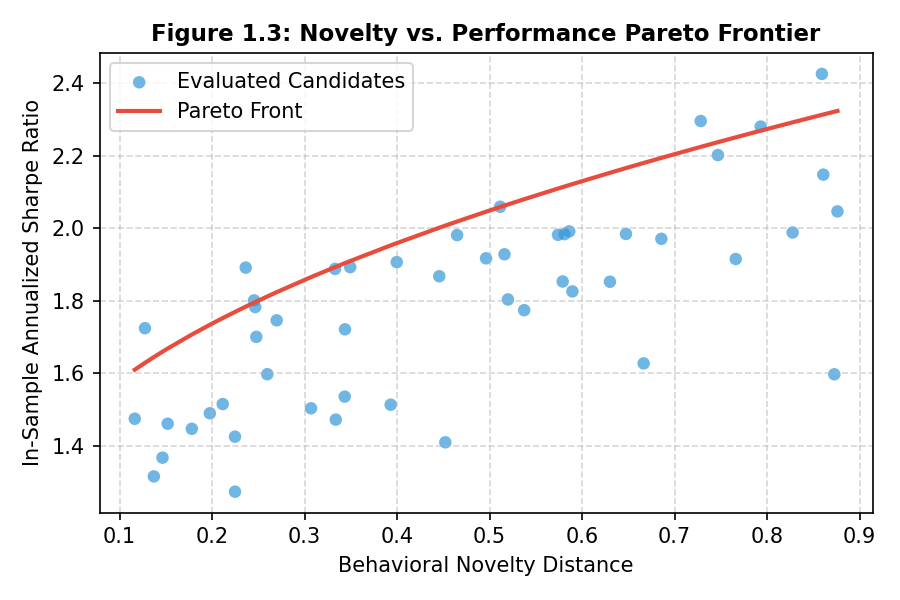
\includegraphics[width=\columnwidth]{../../reports/figures/fig_1_3_pareto_front.png}
\caption{Bi-objective Pareto frontier trading off Novelty Distance against In-Sample Sharpe Ratio.}
\label{fig:pareto}
\end{figure}

\section{Conclusion}
Domain-informed AST grammars coupled with algebraic canonicalization provide a robust, non-redundant framework for automated alpha discovery. Companion papers in this suite address statistical validation \cite{bailey2017probability} and execution microstructure \cite{almgren2000optimal}.

\bibliographystyle{plain}
\bibliography{../references}

\end{document}
